%!TEX root = ../dissertation.tex

\subsection{Wi-Fi (IEEE 802.11)}
\label{subsection:wifi}

A \gls{WLAN} is a wireless network that can connect multiple devices to each other within a limited range. \glspl{WLAN} have become very popular in the day to day life of people. Most households have a \gls{WLAN} deployed so that devices inside and around the premises can have Internet access. The popularity of \glspl{WLAN} is mainly due to the fact that devices do not need to be physically connected to the \gls{AP} to access the Internet, which removes the costs of cables and the associated infrastructures.

IEEE 802.11 is the \textit{de facto} standard for \glspl{WLAN} and it is commonly known as Wi-Fi. IEEE 802.11 is composed by \gls{MAC} layer and Physical layer specifications for \gls{WLAN} implementations, various versions have been released, but the most common are IEEE 802.11a/b/g/n/ac, mainly because they were adopted by mobile and computer manufacturers as the standard to be used in radio communication, \textit{i.e.} wireless.

Unfortunately, the connection speeds are not as high as in wired networks, since the environment plays a big role, \textit{i.e.} if there are obstacles between the \gls{AP} and devices. Also, the number of devices in the network will affect the data speeds, since the protocol specified for the IEEE 802.11 standard is \gls{CSMA/CA}. Although these are disadvantages over wired technologies, there has been done a lot of improvement on the data rates, during the development of wireless networks, reaching up to 6.93Gbps, using \gls{MIMO}, high-order \gls{OFDM} and enhanced \gls{MAC} techniques, see \cite{IEEE80211} for more information on this topic.

In \gls{CSMA/CA} the devices check the medium for clearance, \textit{i.e.} if there is no other device transmitting at that time. Nodes attempt to avoid collisions by transmitting the full data only when the medium is clear. Hidden node is still a problem with this \gls{MAC} method, meaning a node can be transmitting but its transmission is not detected by other devices, creating collisions.

In order to overcome the hidden node problem, \gls{RTS}/\gls{CTS} can be used to reserve the access to the shared medium. A control packet \gls{RTS} is sent by the transmitter, to which the receiver will answer with a \gls{CTS}. If the channel is clear the packet will be sent immediately, \textit{i.e.} if a \gls{CTS} was received, else the device will wait a random period of time, named backoff time, before checking if the medium is clear again. When the backoff timer reaches zero, the device will perform the check, if the medium is clear the device will send the packet, otherwise the backoff time is set again. Due to the exponential factor of this backoff time the connections' speeds are limited when multiple users use exhaustively the network channel, whereas in wired connections, like switched Ethernet, traffic management is, typically, done through traffic flow prioritization.

Another main consequence of establishing a \gls{WLAN} is the security of the communication. In wired networks there is a physical component to security, such as controlled access to the building. In \glspl{WLAN} networks this type of security is not relevant as, for instance, one can enter the network outside the building. Thus security protocols must be implemented to successfully prevent attacks on the communication between devices, such as WPA2 or IEEE 802.11i, see \cite{security} for more information on security protocols.

A \gls{WLAN} can have three different main modes of operation, infrastructure, ad hoc mode and Wi-Fi P2P. Besides these three main modes, IEEE 802.11s will also be briefly explained due to its characteristics and similarities with this work. In the next subsections these modes will be explained, and provided of pros and cons.

\subsubsection{Infrastructure}

Infrastructure is the most common method, usually deployed and made accessible by a local \gls{ISP} or by a Local Area Network. The structure of the network is as follows, there is a wireless \gls{AP} that manages the various devices on the network and provides the Internet access, this \gls{AP} can be either wired, \textit{e.g.} fiber, or wireless connected to network backbone. The \gls{AP} is responsible for the creation and maintenance of the network, it generates an SSID with which the network will be identified, aswell as a security level, \textit{e.g.} \gls{WPA} or \gls{WPS}.

\gls{MS}s can then connect to the network via wireless or wired connections. In the wired connections no authentication is required as there is a physical connection and usually higher data throughput is achieved. In wireless connections there is the need of first identifying the network to which the \gls{MS} wishes to connect and then to proceed according to the security level used by the \gls{AP}. The access to the network is managed by the \gls{AP}, the wired connections are, usually, granted priority over the network, whereas wireless connections compete for the usage of the air interface, typically, via a predefined \gls{MAC} protocol, being the most used \gls{CSMA/CA}.

An example of the infrastructure mode network layout can be seen in Figure \ref{fig:infranet}.

\begin{figure}[ht]
	\noindent\makebox[\textwidth]
    {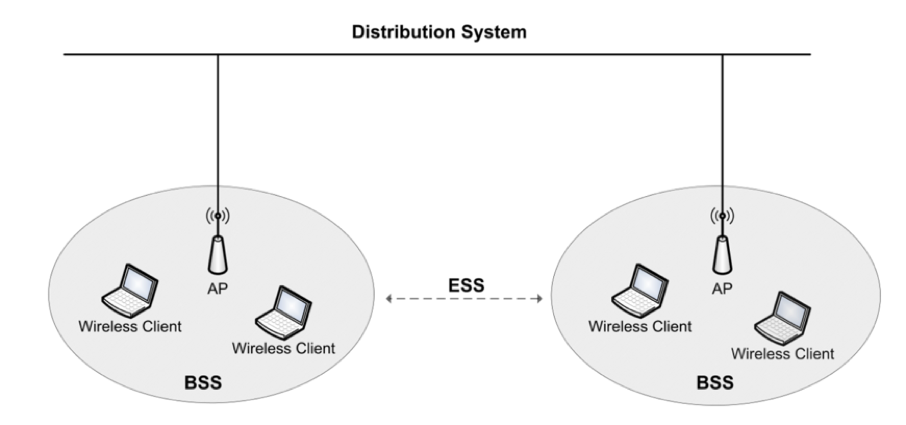
\includegraphics[width=1\textwidth]{images/infranet.png}}
	\caption{\label{fig:infranet} Infrastructure network layout (source: www.cse.wustl.edu)}
\end{figure}

Where each \gls{BSS} is a network and \gls{ESS} is a set of \glspl{BSS} that form a single sub network.

The infrastructure mode is ideal if the network as a more permanent character, since the \glspl{AP} are, usually, developed to provide higher-power wireless radios and antennas so that the area covered by the \glspl{AP} is wider. Despite being the most widely deployed method there are some disadvantages associated with this method, for instance, two \glspl{MS} will not be able to communicate directly even if they reside in the same network, and all their traffic is routed by the \gls{AP}, which brings another problem: in case of \gls{AP} failure due to, \textit{e.g.} power failure, software failure, \textit{etc.}, all the network will be compromised and to establish an Internet connection the \glspl{MS} will have to either connect to another \gls{AP} or to create the connection by themselves, which brings us to the next subsection.

\subsubsection{Ad hoc Networks}

In the ad hoc mode there is no need for a centralized \gls{AP}, meaning all the devices can connect to each other if within range. An ad hoc network is slightly different from a Wi-Fi Direct network (WIFI P2P) that will be described in the next section. In ad hoc mode the network is meshed, and all the devices within it are peers, which brings some benefits, \textit{e.g.} the direct communication between devices, without depending on a centralized point connected to the distribution system.

In ad hoc networks with a mesh topology there can be peer-to-peer exchange of traffic. This helps with the problem of having a centralized point of failure, such as the one present in infrastructure mode. Much like \textit{torrents} files can be transferred by smaller parts and by different providers, by using this method to transfer files, packets, \textit{etc.}, within the network higher data rates can be achieved, since multiple parts of the same file/packet can be sent simultaneously.

An example of the ad hoc mode network with a mesh topology can be seen in Figure \ref{fig:adhocnet}.

\begin{figure}[ht]
	\noindent\makebox[\textwidth]
    {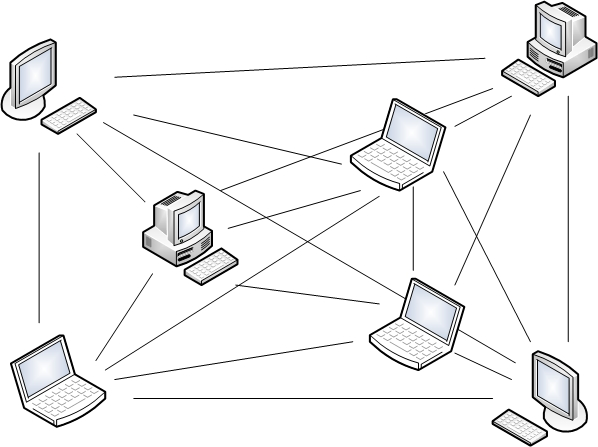
\includegraphics[width=0.5\textwidth]{images/adhocnet.jpg}}
	\caption{\label{fig:adhocnet} Ad hoc network layout (source: monet.postech.ac.kr)}
\end{figure}

As can be seen in Figure \ref{fig:adhocnet}, one device can have multiple links connecting him to other devices in the network. Although this is a big plus if compared with infrastructure mode, it must be noted that, as said before, a device can connect to other devices if in range, otherwise they will not be able to establish a link and thus communicate. This limitation is due to the lack of a routing protocol in this network mode, so nodes cannot serve as relay for communication between two \glspl{STA}, and although it is possible to implement a layer 3 (Network Layer) routing protocol with this mode, such as \gls{AODV}, it is not intrinsic to this mode. In the next subsection, IEEE 802.11s will be introduced and we will see that it covers this limitation of this ad hoc mode.

Although there are advantages such as not having a centralized point of failure, peer-to-peer file/packet transfer described above, there is an easier setup of the network and the problem described in the infrastructure mode of not existing a direct connection between two \glspl{STA} is now mitigated as every \gls{STA} in the network is a peer, there are some disadvantages associated with this network mode, such as the network being more dynamic which brings a lot of changes in the network topology, the interference inherent to all the devices transmitting at the same time to different peers and there is always the scalability problem as more devices in the network mean more connections, which grow exponentially, whereas in the infrastructure mode the connections grow only linearly, so ad hoc networks don't scale well. Also, due to the lack of a routing protocol, the range of the the network will be significantly reduced, as devices do not know which route to forward the packets, in order to reach a certain destination.

Furthermore, the network will not be able to reach the Internet, since devices will communicate between themselves and not with the infrastructure, making the packet exchange limited to the local/cached information stored in the devices, unless if the infrastructure and ad hoc networks are connected through a common device. Finally, the mobility of the devices can make the maintenance of stability of the network a difficult task as links may have to be created and destroyed regularly.

\subsubsection{IEEE 802.11s (Meshed Network)}

IEEE 802.11s is a standard introduced in 2011 which aimed to provide both broadcast and unicast delivery of information. The main difference between the previously described ad hoc mode is that IEEE 802.11s supports multi-hop and implements a layer 2 routing protocol named \gls{HWMP}.

In this standard, four main types of devices exist: \glspl{MP} who establishes peer links with other \glspl{MP}, \glspl{MAP} that is a characteristic of \glspl{MP} which provides \gls{BSS} services to support communication with \glspl{STA}, \glspl{STA} which are devices outside the meshed \gls{WLAN} and connect to the network via \gls{MAP}, finally, \gls{MPP} that is the point at which devices enter and exit the network.

\glspl{MP} discover potential neighbors based on beacon and probe messages, containing the \gls{WLAN} Mesh Capability Element, a summary of active protocols and other channel information, and the Mesh ID, that identifies the mesh. The devices are considered to be members of the network upon the establishment of a secure peer link with neighbors within the network. In Figure \ref{fig:ieee80211s}, taken from \cite{IEEE80211s}, it is possible to visualize an example of the network: 

\begin{figure}[ht]
	\noindent\makebox[\textwidth]
    {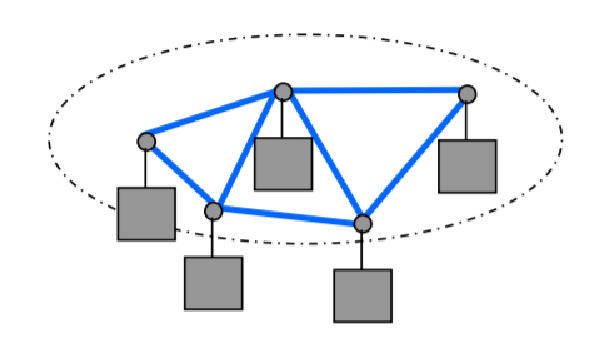
\includegraphics[width=0.7\textwidth]{images/ieee80211s.pdf}}
	\caption{\label{fig:ieee80211s} IEEE 802.11s network layout (source: \cite{IEEE80211s})}
\end{figure}

Depending on the number of radio interfaces the devices have, IEEE 802.11s allows for multi-group formation, where each radio interface of each device is assigned to a different group, called Unified Channel Graph.

The routing protocol used by IEEE 802.11s, \gls{HWMP}, is based on a combination of Radio Metric \gls{AODV} and tree-based routing, which provides great flexibility in changing environments, great efficiency in fixed mesh deployments, and possible extensibility to metrics other than simple number of hops, such as quality of service, load balancing and power-aware. With this features, \gls{HWMP} extinguished many of the ad hoc mode flaws, such as lack of routing protocol and thus inability to perform multi-hop transfer of packets and network range.

Although IEEE 802.11s comes with some benefits, pure ad hoc mode still predominates as the peer-to-peer mode, due to its simplicity. There are still some products that make use of the IEEE 802.11s, such as Linux operating system, FreeBSD operating system and Google WiFi routers.

\subsubsection{Wi-Fi Direct}
\label{subsection:wfd}

Wi-Fi Direct is a Wi-Fi standard created by Wi-Fi Alliance. The previously called Wi-Fi P2P, now Wi-Fi Direct, is an innovative way of mobile communication without the dependence of a physical AP. It can be used for different purposes, such as file transfer, Internet browsing, device communication, \textit{etc.}. Wi-Fi Direct assumes an ad hoc topology, meaning the devices are not dependent on one another, but form a network where all devices share information, hence called peer-to-peer. In Figure \ref{fig:wifidirnet}, it is possible to see the difference between traditional infrastructured Wi-Fi (to the right) and Wi-Fi Direct (to the left).

\begin{figure}[ht]
	\noindent\makebox[\textwidth]
    {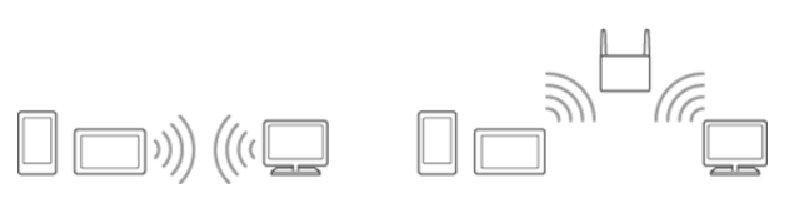
\includegraphics[width=0.7\textwidth]{images/wifidirnet.pdf}}
	\caption{\label{fig:wifidirnet} Wi-Fi Direct (left) and traditional Wi-Fi (right) network layouts (source: info.tvsideview.sony.net)}
\end{figure}

Wi-Fi Direct is not dependent on an infrastructure, meaning even without access to a Wi-Fi network it is possible for devices to connect with each other, this because the Wi-Fi Direct enables devices to emit a signal to other devices in the vicinity announcing the possibility of making a connection. Users in the vicinity of the sending device receive an invitation to join a network (Wi-Fi Direct group).

The process of group creation and administration is the most important topic to this work, regarding this technology. Devices can either join existing groups or create new groups, where they will be the administrators, \textit{a.k.a.} \glspl{GO} of that particular network. This type of creation forces the Wi-Fi Direct to shape its topology as a star, as is evidenced in Figure \ref{fig:wifidirnet}, where there is a central soft \gls{AP}. It is important to make clear the distinction between a soft and a physical \gls{AP}: the physical \gls{AP} usually refers to a physical router, that administrates a network with wired and/or wireless devices, whereas the soft \gls{AP} can be set up with a Wi-Fi adapter, present in many devices, such as mobile phones, computers, \textit{etc.}.

After the creation of a group, the \gls{GO} announces to all nearby devices its group, via the Service Discovery protocol, that sends a beacon packet with an \gls{SSID}, that will be the identifier of the network. Then, the receiving devices can connect to the desired network, by sending information about the device and what type of services it supports. Along with the unique identifier of that device, when received by the \gls{GO}, the devices become \glspl{GM} of that network, much like slaves in Bluetooth, see \ref{subsection:bt}.

In traditional Wi-Fi Direct, the connections are one-to-one or one-to-many, limiting the topology to a star topology, the purpose of this work is to migrate from that star topology to a more dense meshed topology where many-to-many connections are established, and the transfer of data is made faster and without as many relay nodes as in star topology.

The speeds of Wi-Fi Direct are similar to the ones in other Wi-Fi operating modes, reaching up to 250 Mbps. This is the main advantage of Wi-Fi Direct to its direct competitors, such as Bluetooth. As in other wireless technologies, the speed is affected by the environment where the network is inserted, the physical characteristics of the devices and the Wi-Fi physical layer they support, \textit{e.g.}, 802.11a, g or n.

